\section{Estructura de la materia}

La materia está formada por átomos, los átomos están formados por protones, neutrones y electrones.

\sskip
Los protones ($p^+$) tienen carga positiva. Los electrones ($e^-$) carga negativa y los neutrones ($n^0$) no tienen carga.

\sskip
Los átomos son de distintos elementos. Los elementos son los que aparecen en la tabla periódica. El número atómico de un elemento es la cantidad de protones que tiene tal átomo. El número másico de un átomo es la cantidad de protones sumado a la cantidad de neutrones que tiene el átomo. Los átomos cuando se encuentran neutros tienen misma cantidad de electrones que de protones.

\sskip
Cuando un átomo no tiene misma cantidad de electrones que de protones tendrá carga positiva (catión) o negativa (anión). Estos átomos cargados son los \textbf{iones}.

\sskip
Si dos átomos son del mismo elemento (misma cantidad de protones) pero tienen diferente cantidad de neutrones (diferente número másico) estos átomos son distintos \textbf{isótopos} de un mismo elemento.

\subsection*{Propiedades}
\begin{itemize}
    \item El \textbf{radio atómico} es qué tan grande es el átomo. A mayor \textbf{Z} mayor radio atómico.
    \item La \textbf{energía de ionización} es la energía necesaria para desprender un electrón de un átomo neutro en estado gaseoso. Cuanto más a la derecha estés mayor es la energía de ionización (los alcalinos ceden electrones muy fácilmente, los gases nobles casi nunca los ceden). Además a mayor radio atómico menor es la energía de ionización (los electrones están más lejos del núcleo, es más fácil desprenderlos).
    \item La \textbf{afinidad electrónica} es la energía que un átomo libera cuando capta un electrón. En general es proporcional a la energía de ionización, salvo por que los gases nobles no tienen afinidad electrónica.
    \item La \textbf{electronegatividad} es capacidad que tiene un átomo de atraer electrones a sí mismo. También es más o menos proporcional a la energía de ionización y a la afinidad electrónica, aunque está llena de excepciones. Es una de las propiedades que aparece en la tabla periódica. Los elementos más electronegativos son el flúor, oxígeno, cloro y nitrógeno.
\end{itemize}

\subsection*{Tabla periódica}

Dentro de la tabla periódica cada elemento tiene su \textbf{número atómico ``Z''}, su \textbf{número másico ``A''}, su \textbf{masa atómica} y su \textbf{símbolo}. 

\sskip
Las diferentes columnas se llaman \textbf{grupos} y las filas \textbf{períodos}.
Algunos grupos tienen nombres particulares: grupo 1 son los metales alcalinos, grupo 2 metales alcalinotérreos, grupos 3 a 12 metales de transición, grupo 14 carbonoideos, grupo 15 nitrogenoideos, grupo 16 anfígenos,  grupo 17 halógenos y grupo 18 gases nobles. Los lantánidos y actínidos se dice que son de transición interna.

\sskip
\textbf{Bloques} son los s: primeras dos columnas más helio; p: no metales, metaloides y metales pobres; d: metales de transición; f: lantánidos y actínidos.

\sskip
\textbf{Masa atómica relativa}: es cuánto pesa en promedio un mol de átomos, siendo que los átomos son de distintos isótopos.

\subsection*{Uniones entre átomos}

Los átomos se pueden enlazar con enlaces \textbf{covalentes} (NM+NM), \textbf{iónicos} (M+NM) y \textbf{metálicos} (M+M). 

\sskip 
Los enlaces covalentes forman \textbf{moléculas}, que pueden ser simples (un solo elemento) o compuestas (más de un elemento); los enlaces iónicos generan \textbf{redes cristalinas iónicas} y los enlaces metálicos \textbf{redes cristalinas metálicas}. Las sustancias formadas por un solo átomo se llaman monoatómicas (gases nobles).

\subsection*{Configuración electrónica}

Recordar que dentro de un átomo, los electrones se ubican en orbitales. Los orbitales pueden ser de distintos tipos (S, P, D, F) y estar en diferentes niveles de energía (1, 2, 3, 4, 5, 6 y 7).

\sskip
\textbf{CE}: La configuración electrónica muestra cuántos electrones ocupan los diferentes orbitales.

\textbf{CEE}: La configuración electrónica externa muestra solo la capa más externa de orbitales, básicamente agarrás solo los que están después del gas noble anterior.

\textbf{CES}: La configuración electrónica simplificada es decir cuál es el gas noble anterior y sumarle la CEE.

\begin{figure}[H]
    \centering
    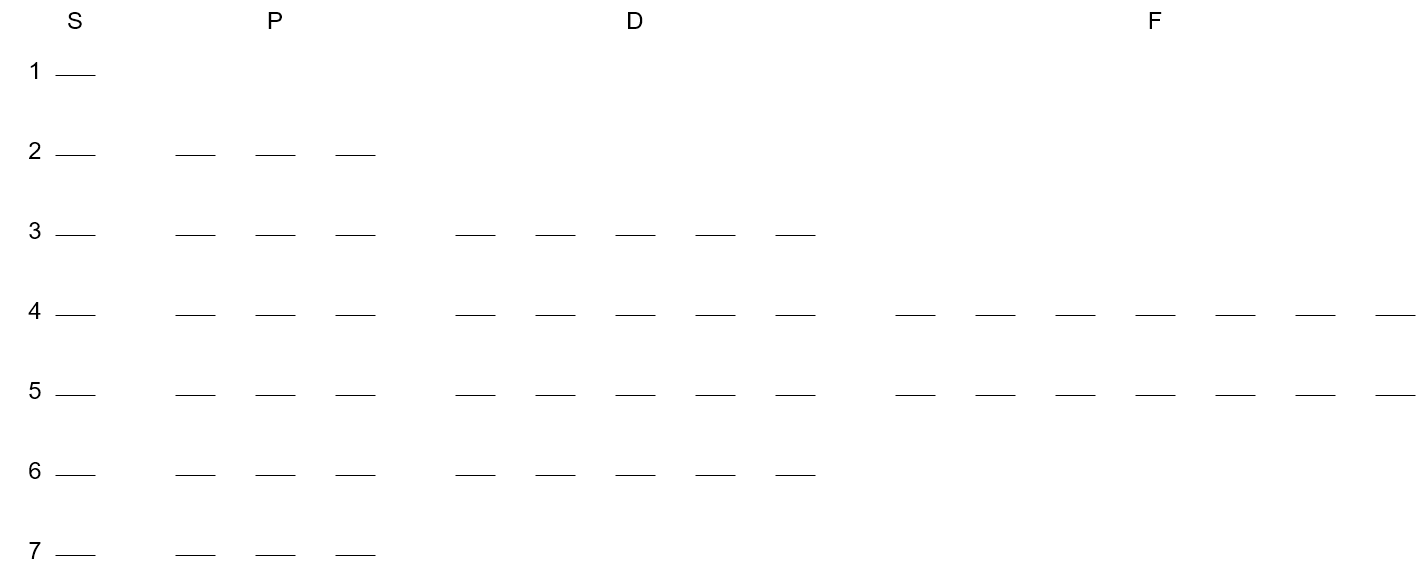
\includegraphics[width=0.8\linewidth]{Images/Orbitales.png}
\end{figure}

